% style/preamble throws error, hence preamble4tex is kept here
\documentclass[11pt,compress,t,notes=noshow]{beamer}\usepackage[]{graphicx}\usepackage[]{color}

\makeatletter
\def\maxwidth{ %
  \ifdim\Gin@nat@width>\linewidth
    \linewidth
  \else
    \Gin@nat@width
  \fi
}
\makeatother

\definecolor{fgcolor}{rgb}{0.345, 0.345, 0.345}
\newcommand{\hlnum}[1]{\textcolor[rgb]{0.686,0.059,0.569}{#1}}%
\newcommand{\hlstr}[1]{\textcolor[rgb]{0.192,0.494,0.8}{#1}}%
\newcommand{\hlcom}[1]{\textcolor[rgb]{0.678,0.584,0.686}{\textit{#1}}}%
\newcommand{\hlopt}[1]{\textcolor[rgb]{0,0,0}{#1}}%
\newcommand{\hlstd}[1]{\textcolor[rgb]{0.345,0.345,0.345}{#1}}%
\newcommand{\hlkwa}[1]{\textcolor[rgb]{0.161,0.373,0.58}{\textbf{#1}}}%
\newcommand{\hlkwb}[1]{\textcolor[rgb]{0.69,0.353,0.396}{#1}}%
\newcommand{\hlkwc}[1]{\textcolor[rgb]{0.333,0.667,0.333}{#1}}%
\newcommand{\hlkwd}[1]{\textcolor[rgb]{0.737,0.353,0.396}{\textbf{#1}}}%
\let\hlipl\hlkwb

\usepackage{framed}
\makeatletter
\newenvironment{kframe}{%
 \def\at@end@of@kframe{}%
 \ifinner\ifhmode%
  \def\at@end@of@kframe{\end{minipage}}%
  \begin{minipage}{\columnwidth}%
 \fi\fi%
 \def\FrameCommand##1{\hskip\@totalleftmargin \hskip-\fboxsep
 \colorbox{shadecolor}{##1}\hskip-\fboxsep
     \hskip-\linewidth \hskip-\@totalleftmargin \hskip\columnwidth}%
 \MakeFramed {\advance\hsize-\width
   \@totalleftmargin\z@ \linewidth\hsize
   \@setminipage}}%
 {\par\unskip\endMakeFramed%
 \at@end@of@kframe}
\makeatother

\definecolor{shadecolor}{rgb}{.97, .97, .97}
\definecolor{messagecolor}{rgb}{0, 0, 0}
\definecolor{warningcolor}{rgb}{1, 0, 1}
\definecolor{errorcolor}{rgb}{1, 0, 0}
\definecolor{code}{rgb}{0.97, 0.96, 1.0}
\newenvironment{knitrout}{}{} % an empty environment to be redefined in TeX

\usepackage{alltt}
\usepackage[utf8]{inputenc}
\usepackage[ngerman]{babel}
\usepackage{dsfont}
\usepackage{verbatim}
\usepackage{amsmath}
\usepackage{amsfonts}
\usepackage{mathtools}
\usepackage{csquotes}
\usepackage{cmbright}
\usepackage{multirow}
\usepackage{longtable}
\usepackage{enumerate}
\usepackage[absolute,overlay]{textpos}
\usepackage{psfrag}
\usepackage{algorithm}
\usepackage{algpseudocode}
\usepackage{eqnarray}
\usepackage{bytefield}
\usepackage{animate}
\usepackage{tikz}
\usetikzlibrary{shapes,matrix,positioning,chains,arrows,shadows,decorations.pathmorphing,fit,backgrounds}
\usepackage{adjustbox}
\usepackage{colortbl}
\usepackage{tabularx} % for tables (incl. \hline)
\usepackage{arydshln} % Load after array, longtable, colortab and/or colortbl , otherwise problems with \hline in tabular env
\usepackage{etex} %increase registers for \dimenS to more than 256, otherwise we get "No room for a new \dimen"
\usepackage{graphicx}
\usepackage{booktabs} %used in epr lectures
\usepackage{bm} % bold greek letters
\usepackage{hyperref} % url citing
\usepackage{blkarray} % block arrays
\usepackage{listings} % block of code
\usepackage{xcolor} %colored math symbols
\usepackage{pgffor}
\usepackage{verbatimbox}
\usepackage{xcolor}

%some colors
\definecolor{checkgreen}{HTML}{18A126}
\definecolor{errorred}{HTML}{FF0000}
\definecolor{blockbg}{HTML}{F7F7F7}
\definecolor{gray}{HTML}{A0A0A0}

% basic latex stuff
\newcommand{\col}{\par\colorbox{code}{\parbox{\textwidth}{\theverbbox}}\par}
\newcommand{\eg}{e.\,g.\xspace} %for example
\newcommand{\ie}{i.\,e.\xspace} %that is to say...
\newcommand{\pkg}[1]{{\fontseries{b}\selectfont #1}} %fontstyle for R packages
\newcommand{\lz}{\vspace{0.5cm}} %vertical space
\newcommand{\oneliner}[1] % Oneliner for important statements
{\begin{block}{}\begin{center}\begin{Large}#1\end{Large}\end{center}\end{block}}
\def\SpAr{\quad \Rightarrow \quad}

%new environments
\newenvironment{vbframe}  %frame with breaks and verbatim
{
 \begin{frame}[containsverbatim,allowframebreaks]
}
{
\end{frame}
}

\newenvironment{vframe}  %frame with verbatim without breaks (to avoid numbering one slided frames)
{
 \begin{frame}[containsverbatim]
}
{
\end{frame}
}

\newenvironment{blocki}[1]   % itemize block
{
 \begin{block}{#1}\begin{itemize}
}
{
\end{itemize}\end{block}
}

\newenvironment{fragileframe}[2]{  %fragile frame with framebreaks
\begin{frame}[allowframebreaks, fragile, environment = fragileframe]
\frametitle{#1}
#2}
{\end{frame}}

\newcommand{\myframe}[2]{  %short for frame with framebreaks
\begin{frame}[allowframebreaks]
\frametitle{#1}
#2
\end{frame}}

\usepackage{../../style/lmu-lecture}

\let\code=\texttt
\let\proglang=\textsf

\setkeys{Gin}{width=0.9\textwidth}

\usepackage{tikz}
\usetikzlibrary{shapes,arrows,snakes, calc}

% Define block styles
\tikzstyle{decision} = [diamond, draw, text width=6em, text badly centered, node distance=4cm, inner sep=0pt]
\tikzstyle{decision2} = [diamond, draw, fill=customgreen!35, text width=6em, text badly centered, node distance=4cm, inner sep=0pt]

\tikzstyle{block} = [rectangle, draw, text width=14em, text centered, rounded corners, node distance=3cm, minimum height=4em]
\tikzstyle{line} = [draw, -latex']
\tikzstyle{cloud} = [draw, ellipse, node distance=3cm, minimum height=2em]

\title{Introduction to Deep Learning}
\author{Bernd Bischl}
\institute{Department of Statistics -- LMU Munich}
\date{WS 2021/2022}

\setbeamertemplate{frametitle}{\expandafter\uppercase\expandafter\insertframetitle}

\IfFileExists{upquote.sty}{\usepackage{upquote}}{}
\input{../../latex-math/basic-math}
\input{../../latex-math/basic-ml}
\input{../../latex-math/ml-nn}

\newcommand{\titlefigure}{figure/alexnet.jpg}
\newcommand{\learninggoals}{
  \item Architecture
}

\title{Deep Learning}
\date{}

\begin{document}

\lecturechapter{CNN: Architecture}
\lecture{I2DL}

%%%%%%%%%%%%%%%%%%%%%%%%%%%%%%%%%%%%%%%%%%%%%%%%%%%%%%%%%%%%%%%%%%
\section{Different Perspectives of CNNs}
%%%%%%%%%%%%%%%%%%%%%%%%%%%%%%%%%%%%%%%%%%%%%%%%%%%%%%%%%%%%%%%%%%
\begin{vbframe}{CNNs - Perspective I}
\center
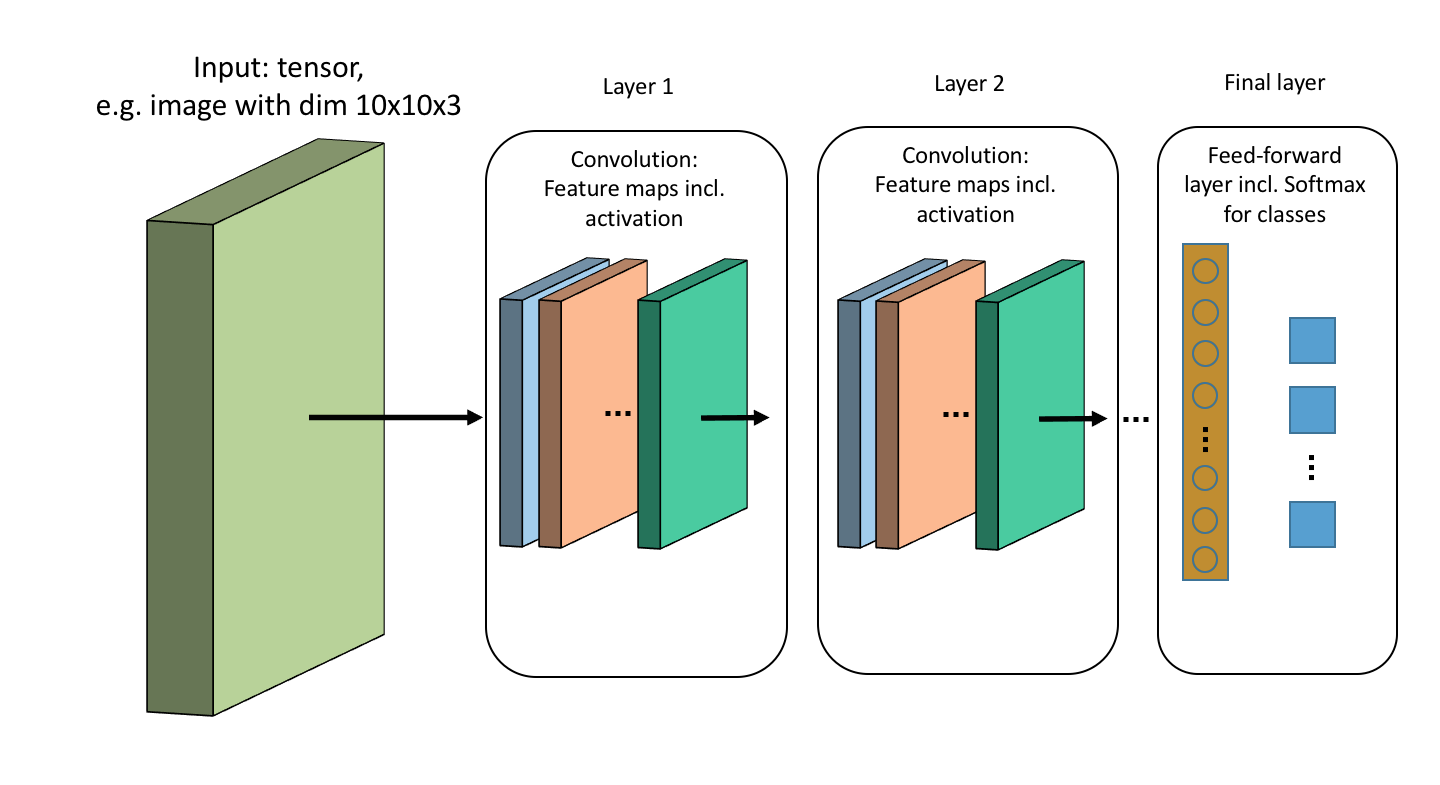
\includegraphics[width=9cm]{figure/cnn_scheme.png}
\begin{itemize}
\item Schematic architecture of a CNN.
\item The input tensor is convolved by different filters yielding different feature maps (coloured) in subsequent layers.
\item A dense layer connects the final feature maps with the softmax-activated output neurons.
\end{itemize}
\end{vbframe}

\begin{vbframe}{CNNs - Perspective II}
\center
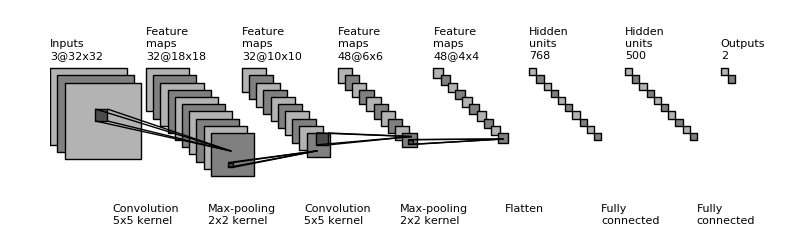
\includegraphics[width=11cm]{figure/cnn_flat.png}
\begin{itemize}
\item Flat view of a CNN architecture for a classification problem.
\item Consists of 2 CNN layers that are each followed by max-pooling, then flattened and connected with the final output neurons via a dense layer.
\end{itemize}
\end{vbframe}

\begin{vbframe}{CNNs - Perspective III}
\center
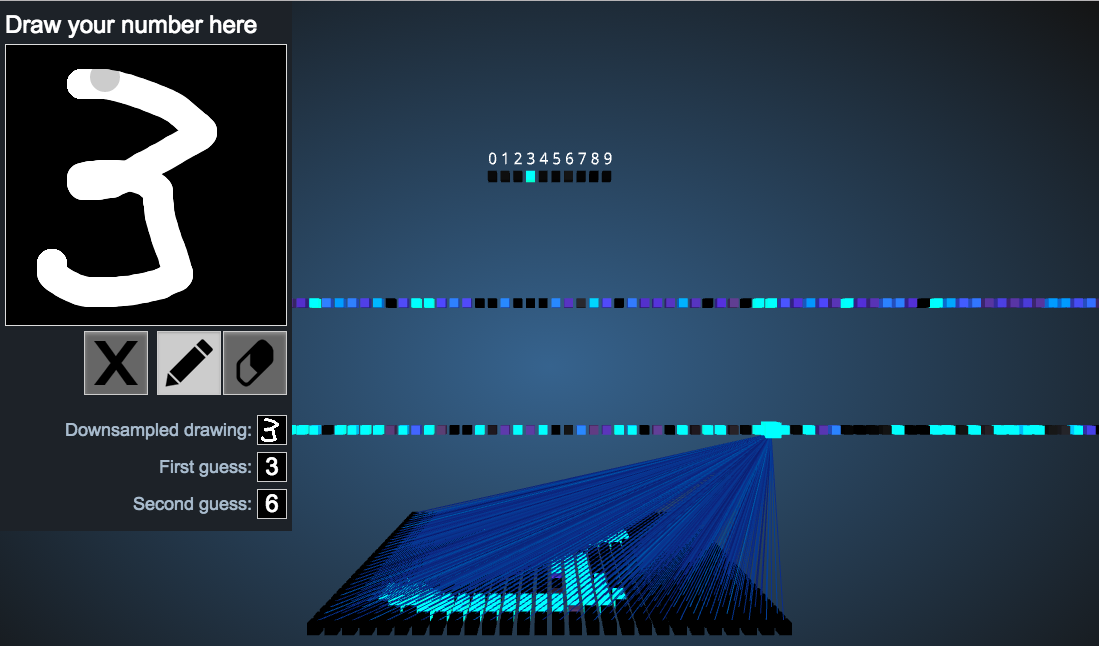
\includegraphics[width=8cm]{figure/3dviz_fcn.png}
\begin{itemize}
% \item Awesome interactive visualization by \cite{29} (\href{http://scs.ryerson.ca/~aharley/vis/}{click here})
\item Awesome interactive visualization (by Adam Harley)  \href{http://scs.ryerson.ca/~aharley/vis/}{\beamergotobutton{Click here}}.
\item Vanilla 2-layer densely-connected net on MNIST data for input digit $3$.
\item Each neuron in layer 1 is connected to each of the input neurons.
\end{itemize}
\framebreak
\center
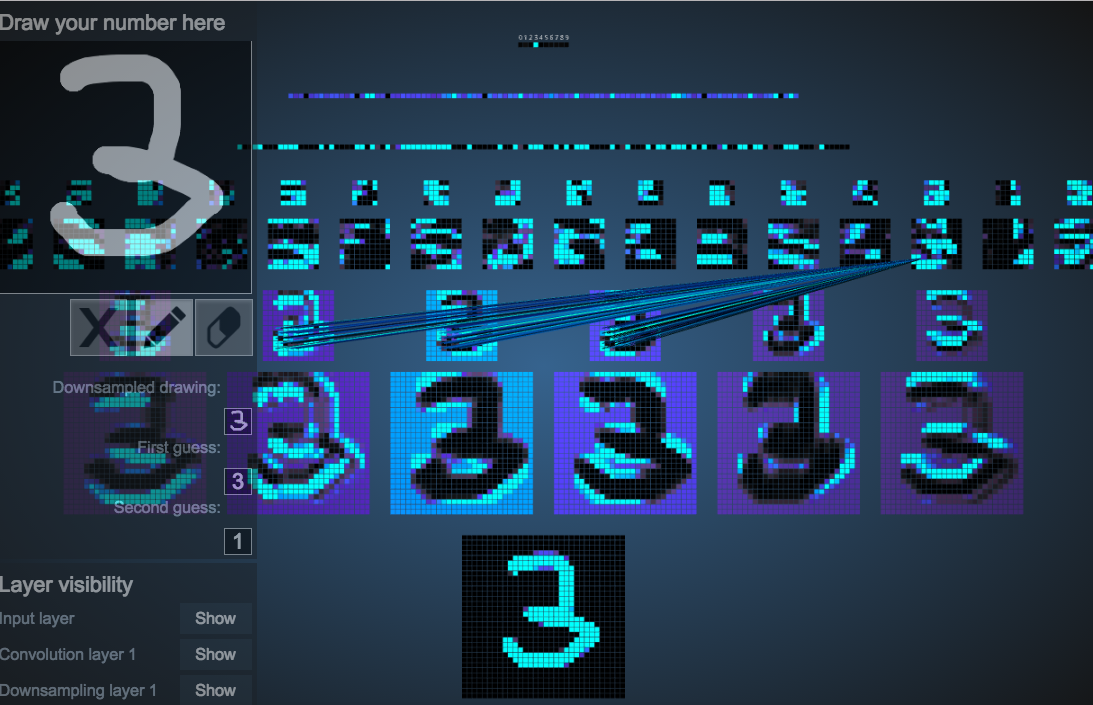
\includegraphics[width=8cm]{figure/3dviz_cnn_front.png}
\begin{itemize}
\item Front view on 2-layer CNN with Pooling and final dense layer on MNIST data for input digit $3$.
\item Each neuron in the second CNN layer is connected to a patch of neurons from each of the previous feature maps via the convolutional kernel.
\end{itemize}
\framebreak
\center
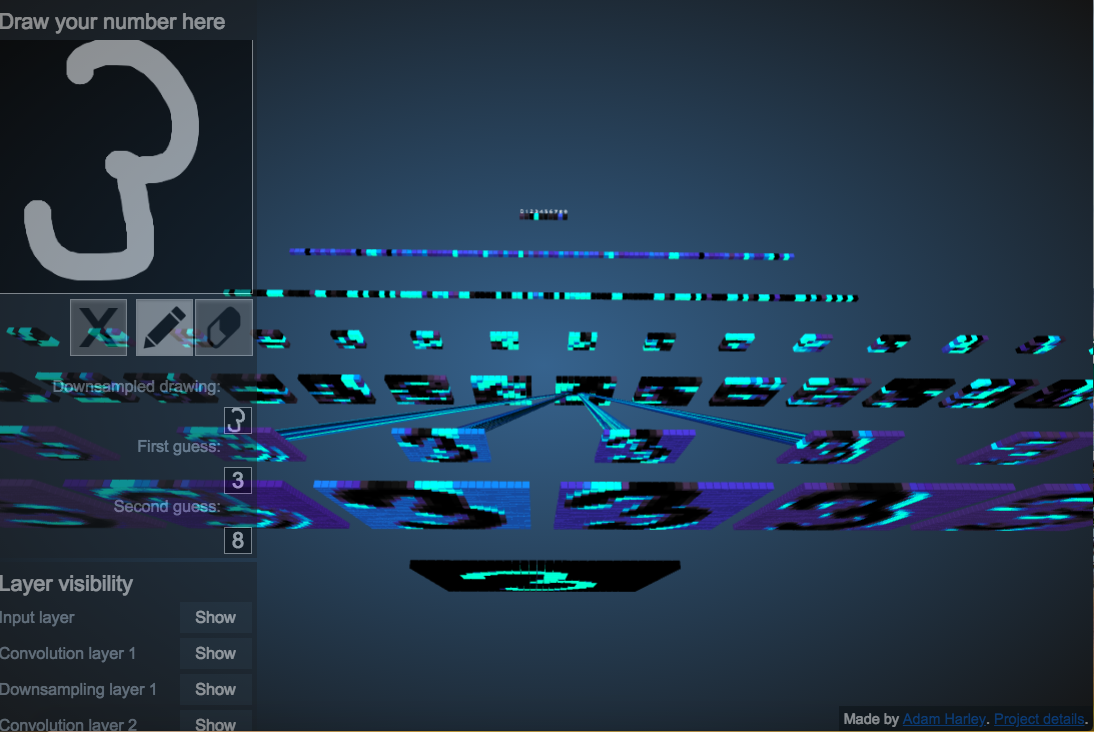
\includegraphics[width=7.5cm]{figure/3dviz_cnn_bottom.png}
\begin{itemize}
\item Bottom view on 2-layer CNN with Pooling and final dense layer on MNIST data for input digit $3$.
\item Each neuron in the second CNN layer is connected to a patch of neurons from each of the previous feature maps via the convolutional kernel.
\end{itemize}
\end{vbframe}



\frame{
    \frametitle{CNNs - Architecture}
    
    \center
    %\only<1>{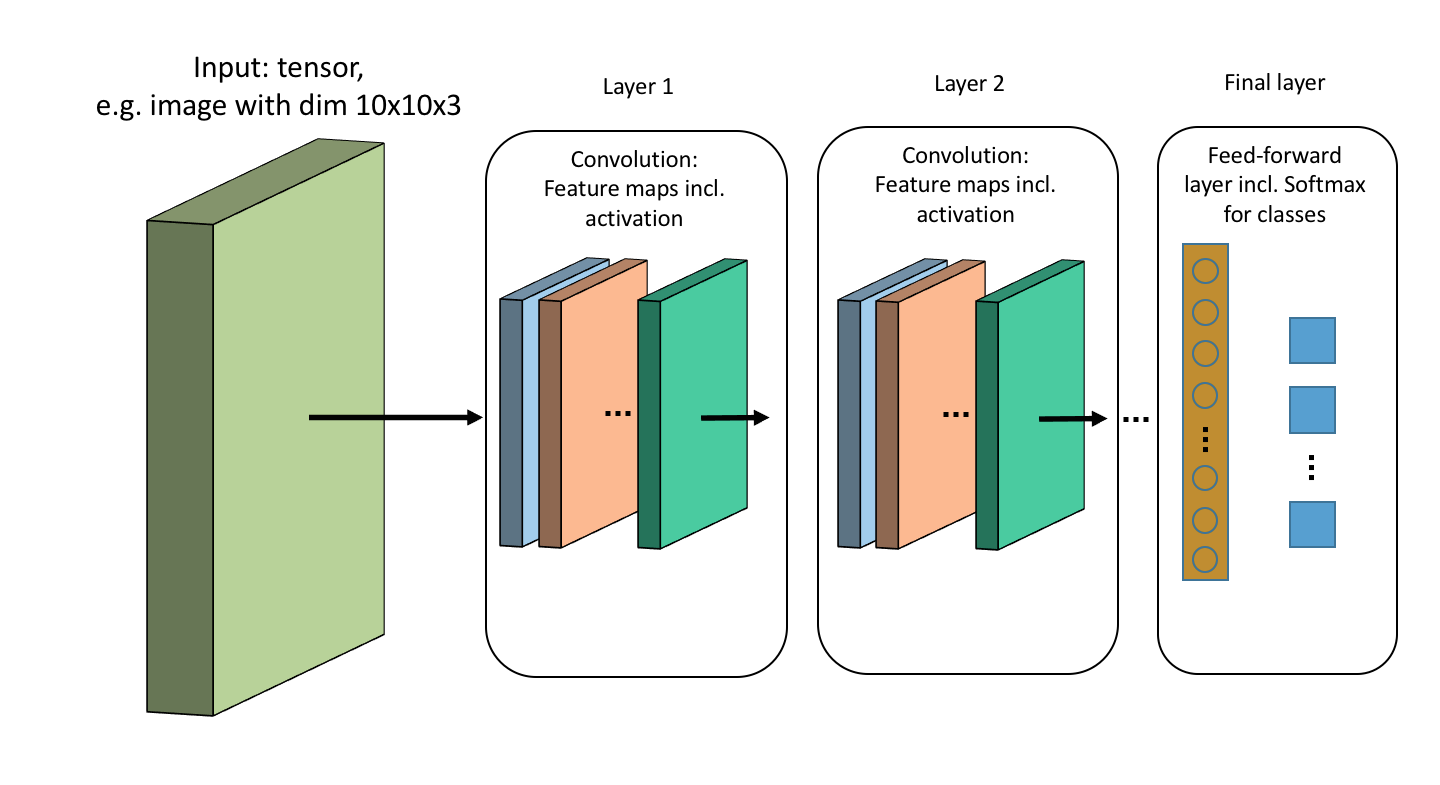
\includegraphics[width=11cm]{figure/cnn_scheme.png}}%
        \only<1>{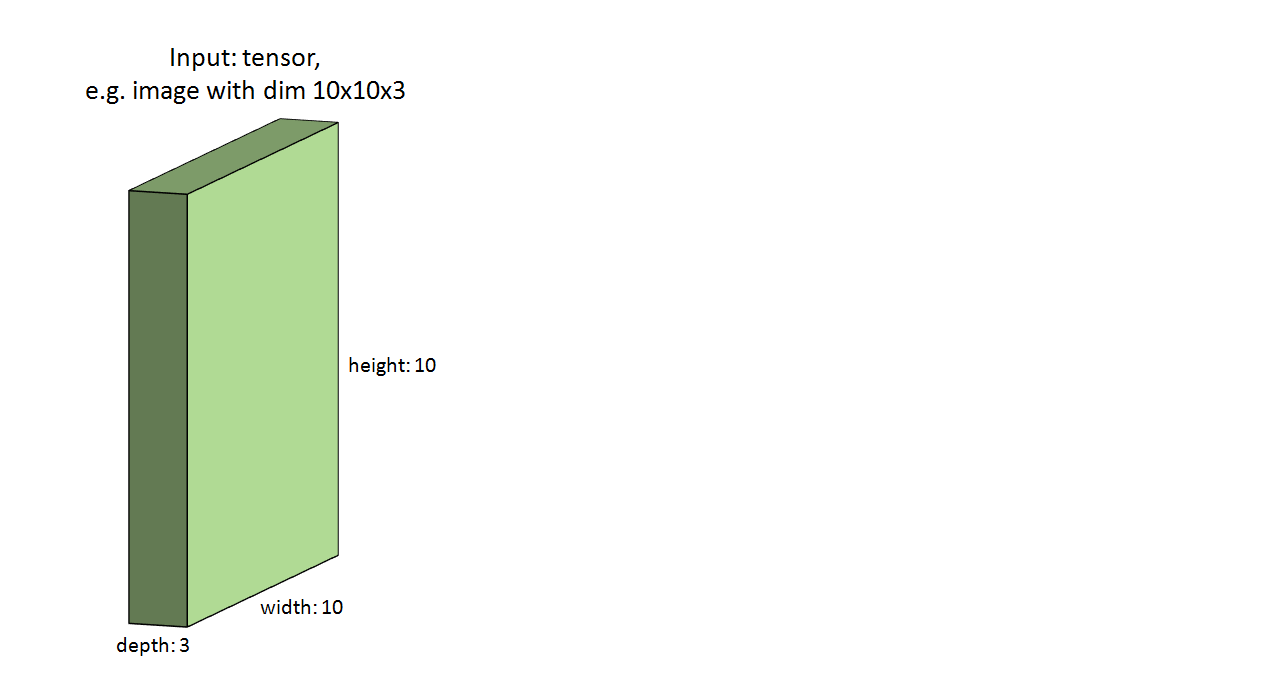
\includegraphics[width=11cm]{figure/cnn1}}%
    \only<2>{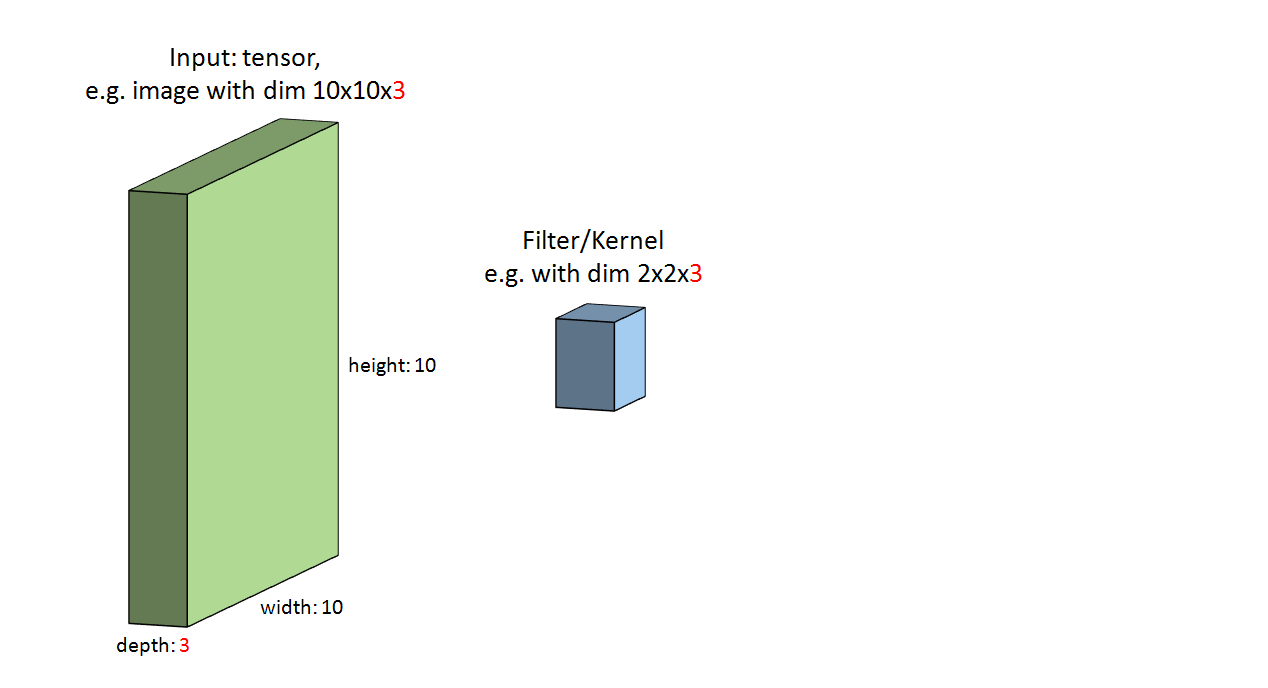
\includegraphics[width=11cm]{figure/cnn2}}%
    \only<3>{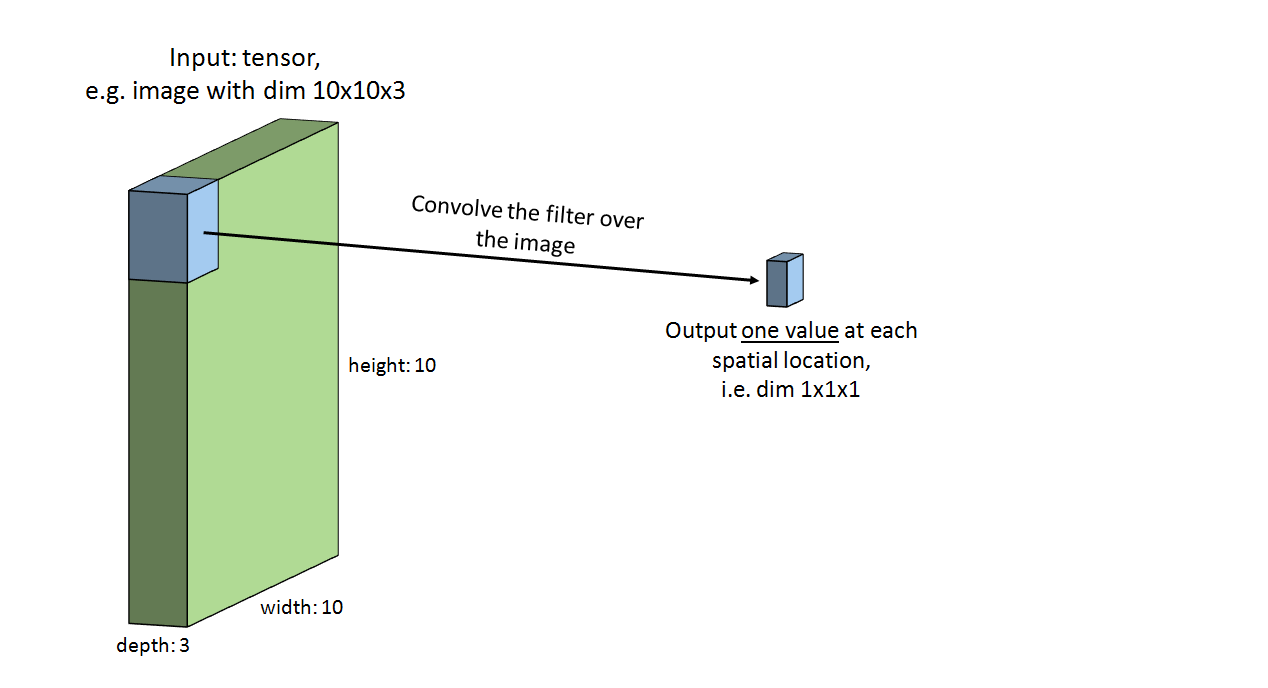
\includegraphics[width=11cm]{figure/cnn3}}%
    \only<4>{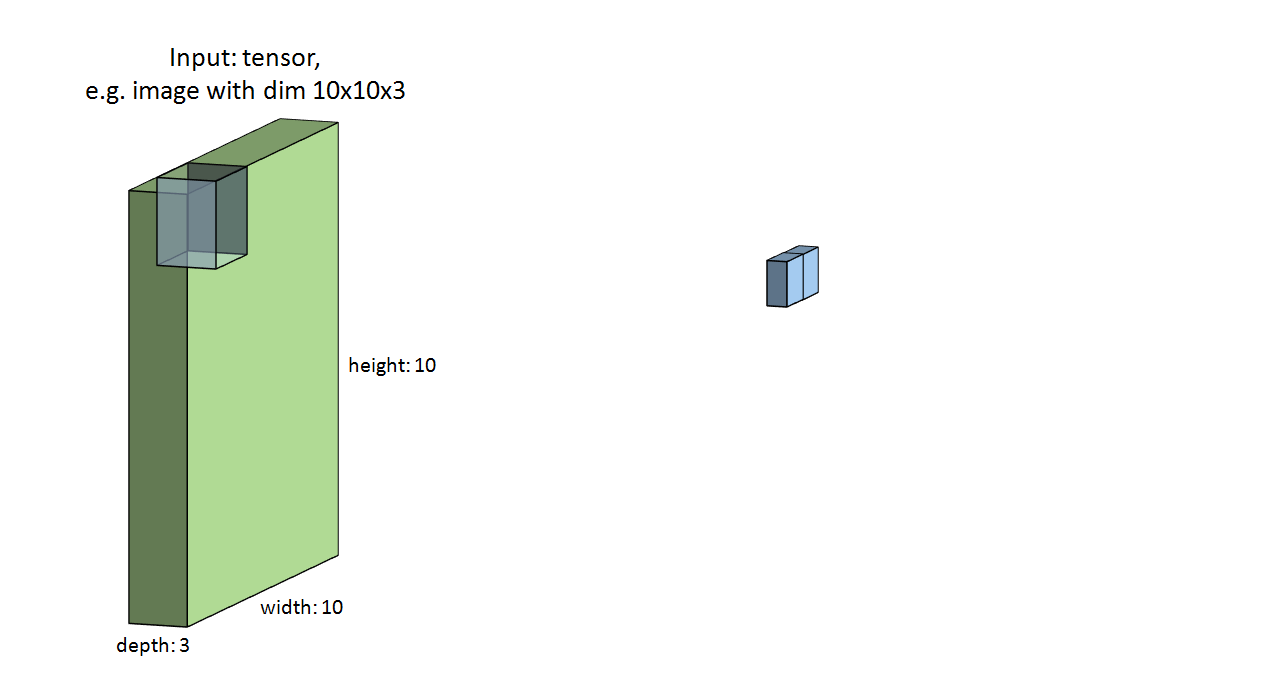
\includegraphics[width=11cm]{figure/cnn4}}%
    \only<5>{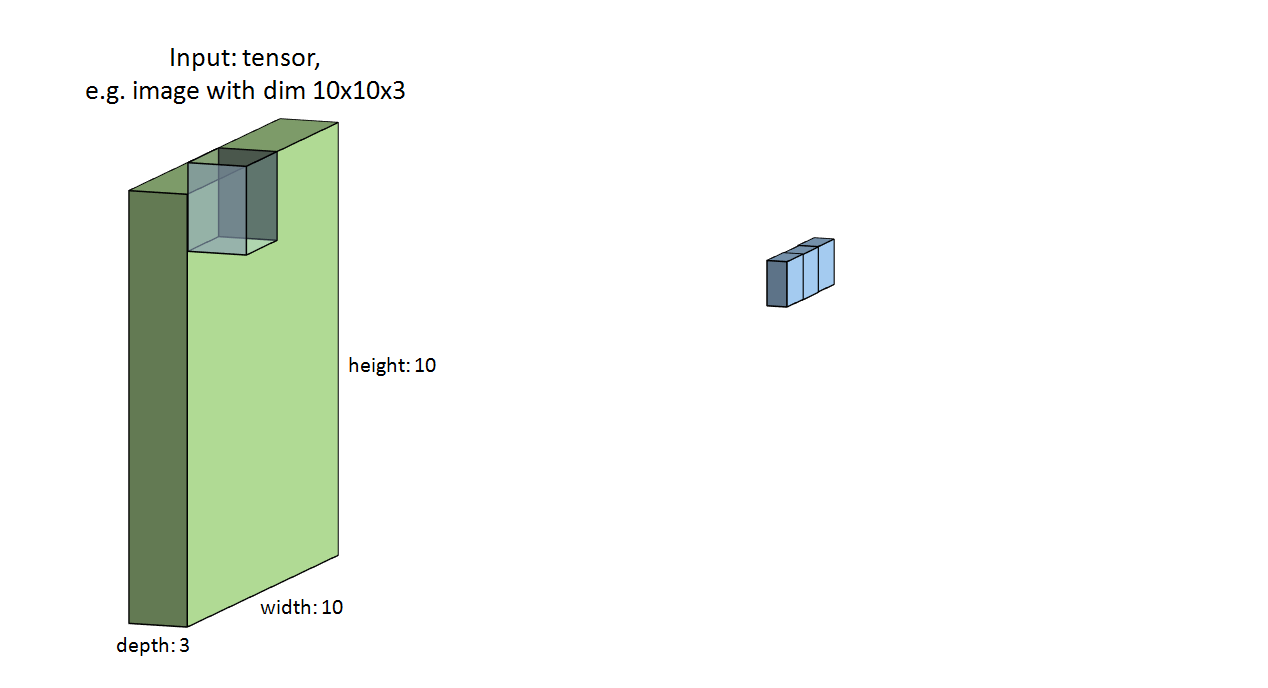
\includegraphics[width=11cm]{figure/cnn5}}%
    \only<6>{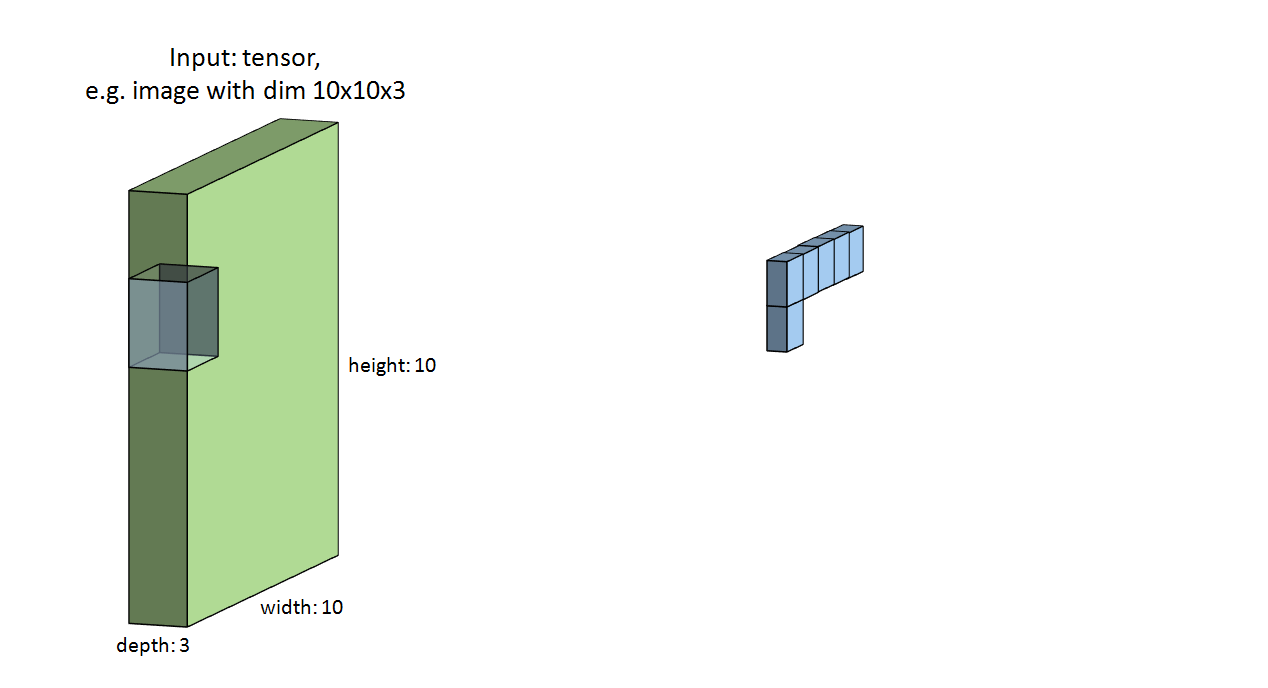
\includegraphics[width=11cm]{figure/cnn6}}%
    \only<7>{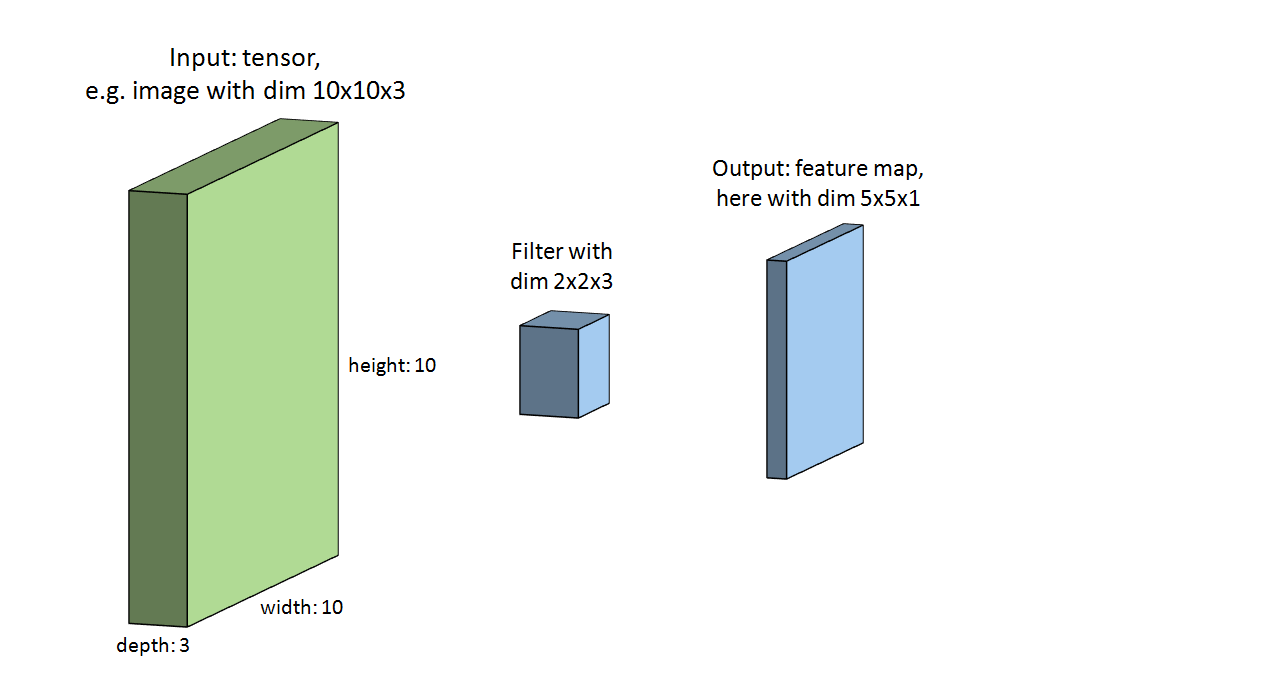
\includegraphics[width=11cm]{figure/cnn7}}%
    \only<8>{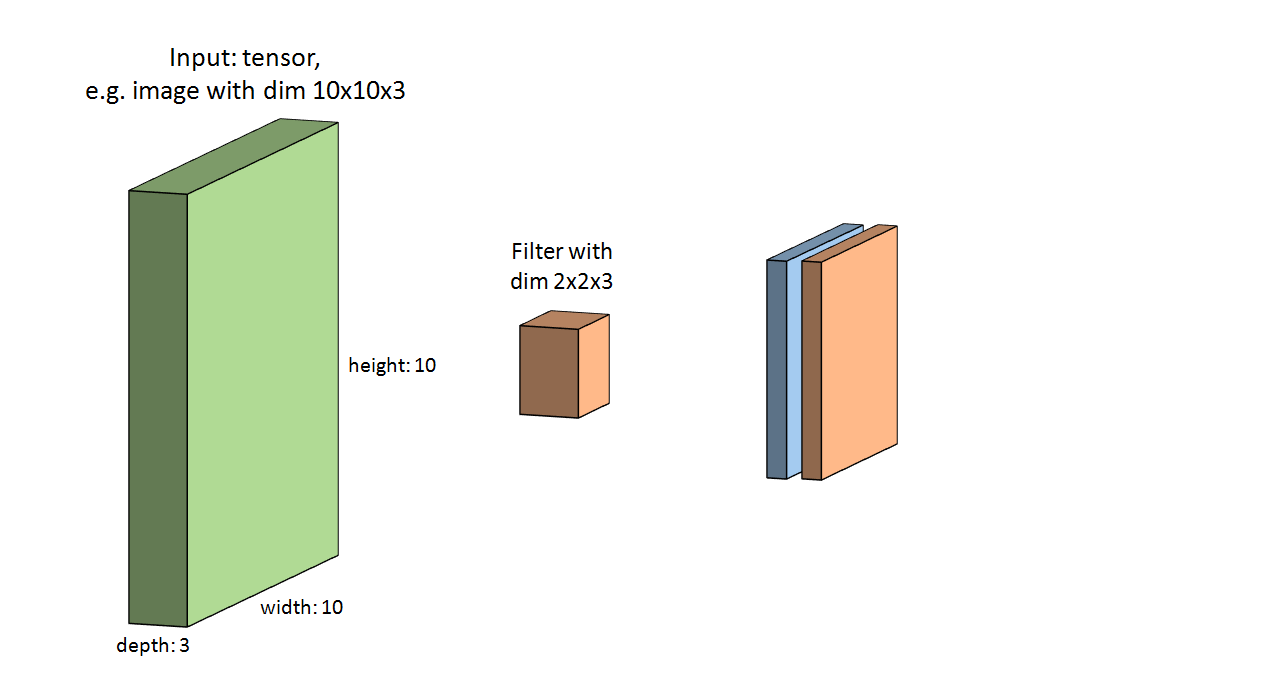
\includegraphics[width=11cm]{figure/cnn8}}%
    \only<9>{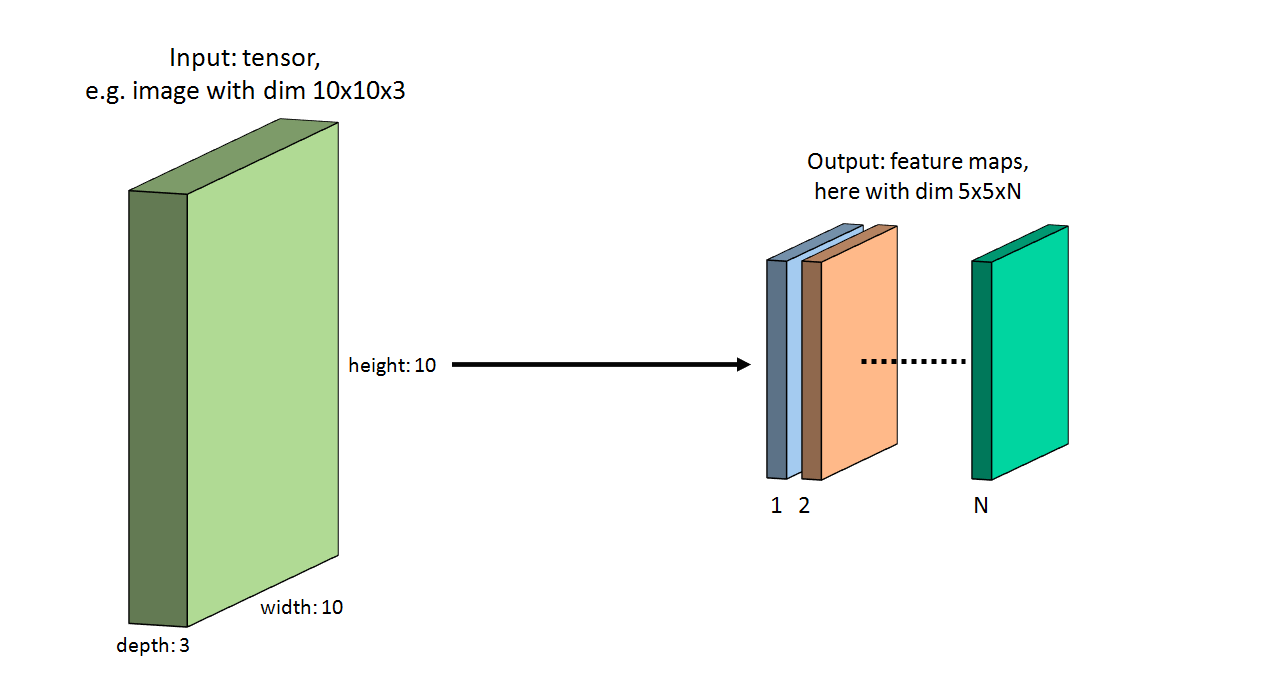
\includegraphics[width=11cm]{figure/cnn9}}%
    \only<10>{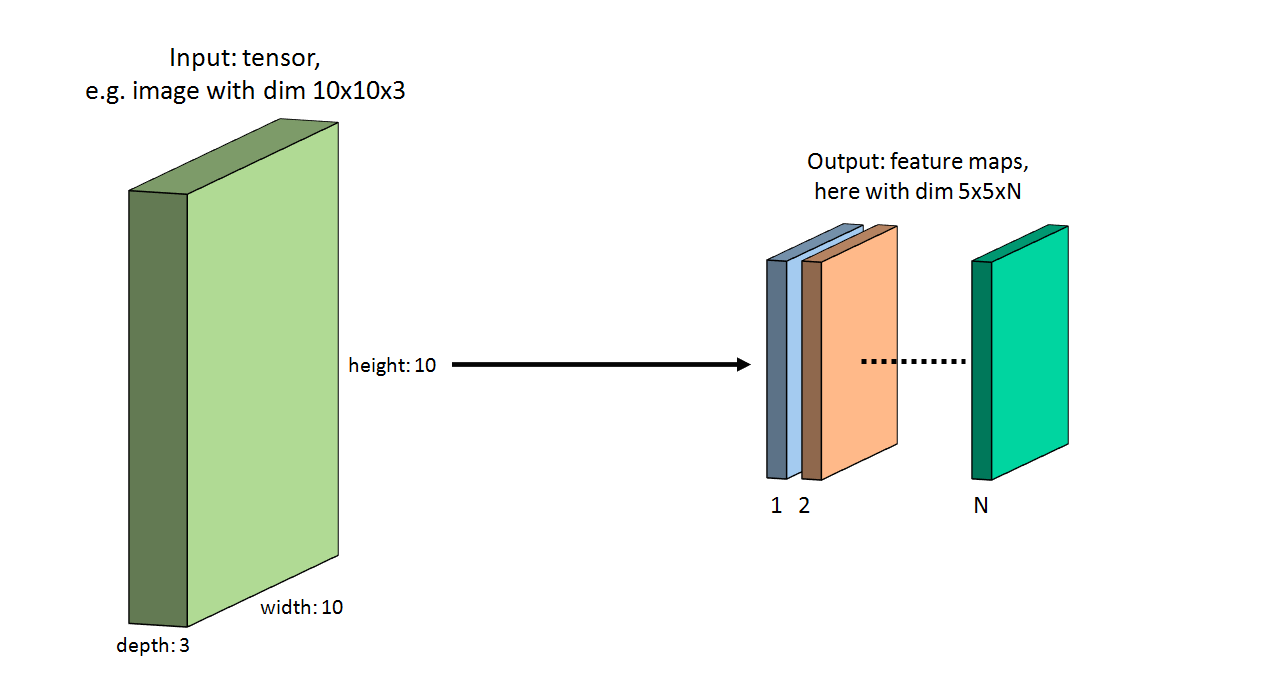
\includegraphics[width=11cm]{figure/cnn9}}%
    \only<11>{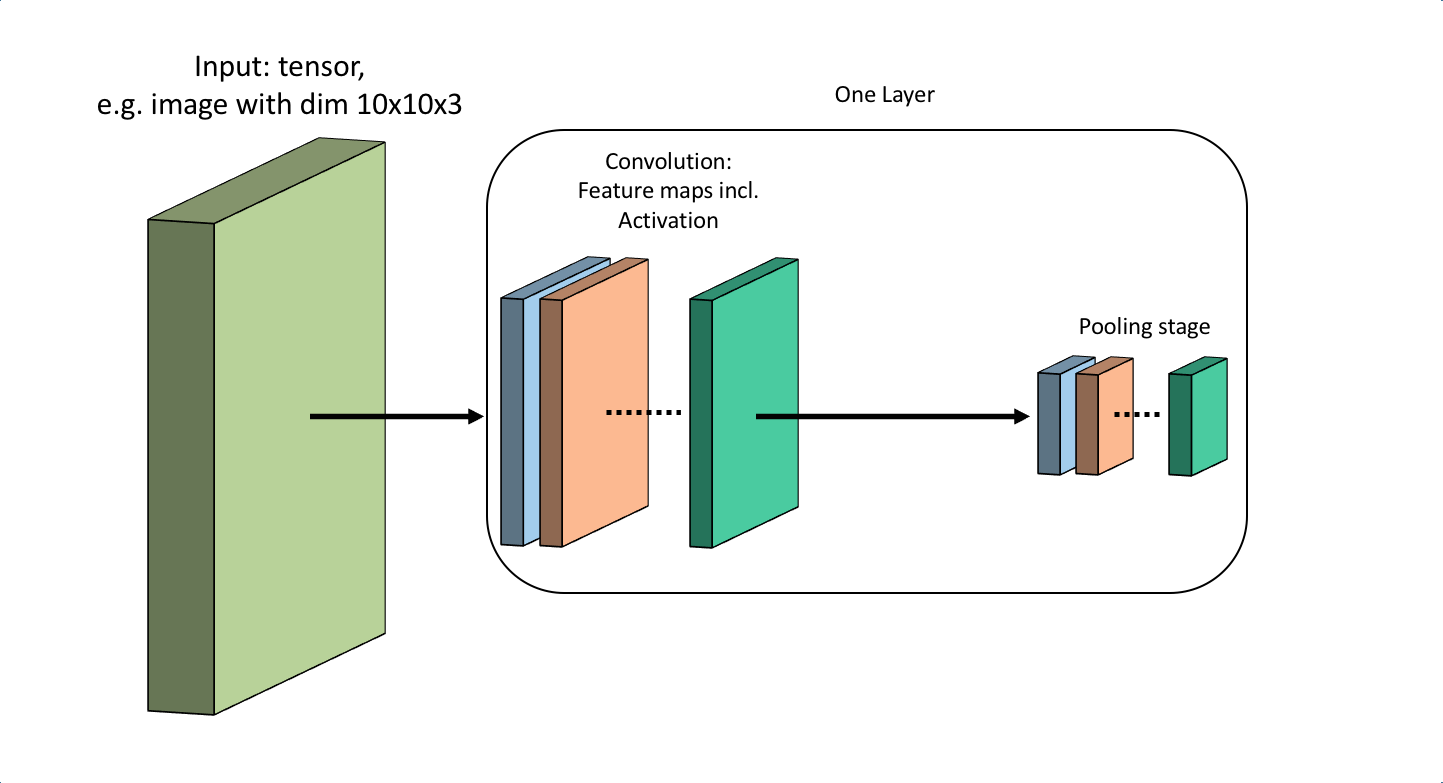
\includegraphics[width=11cm]{figure/cnn11}}%
    \only<12>{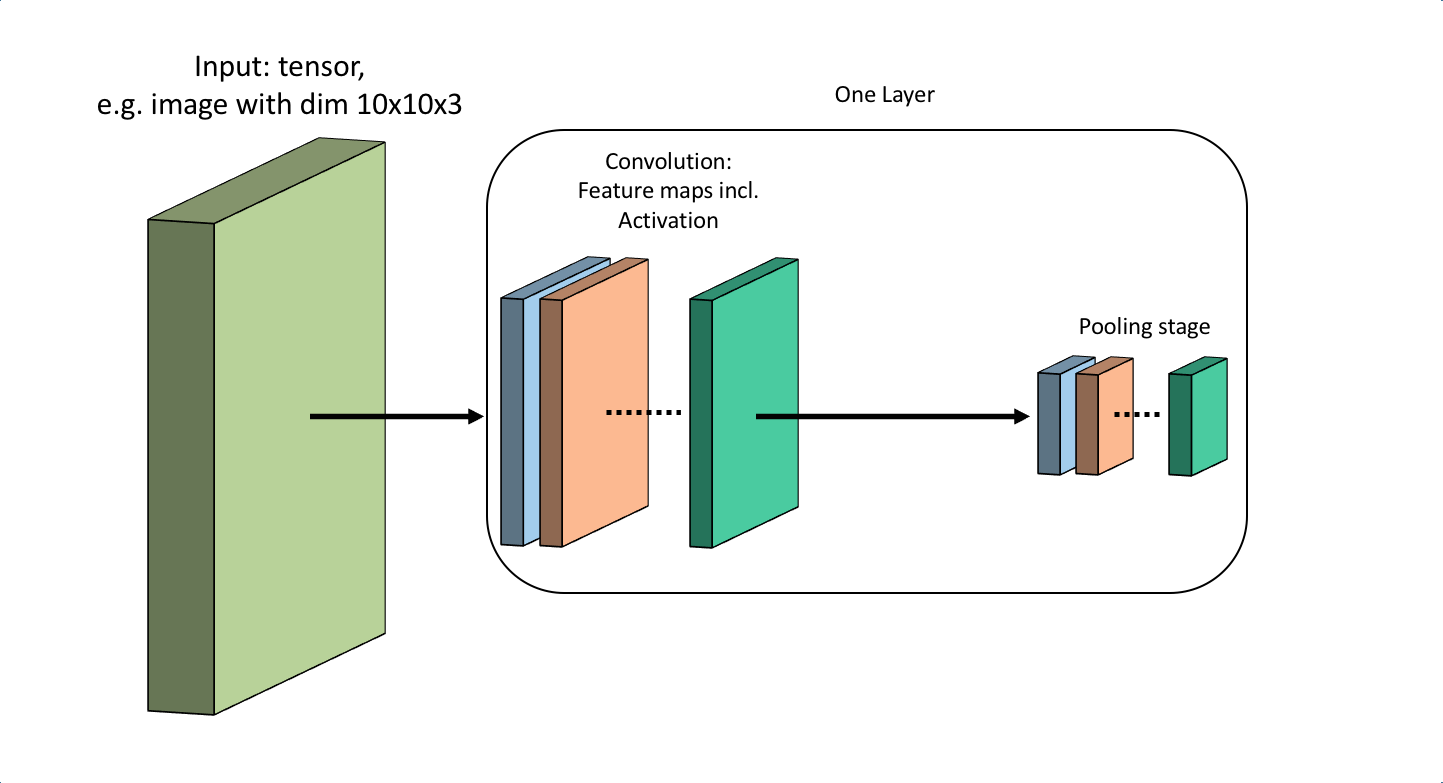
\includegraphics[width=11cm]{figure/cnn11}}%
    \only<13>{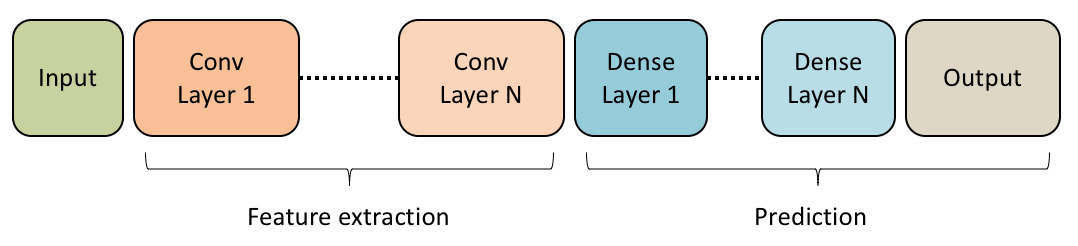
\includegraphics[width=11cm]{figure/cnn12}}%
    
    \begin{itemize}
    %\only<1>{\item Schematic architecture of a CNN}
    \only<1>{\item Suppose we have the following input tensor with dimensions $10 \times 10 \times 3$.}
    \only<2>{\item We use a filter of size $2$.}
    \only<3>{\item Applying it to the first spatial location, yields one scalar value.}
    \only<4>{\item The second spatial location yields another one..}
    \only<5>{\item ...and another one...}
    \only<6>{\item ...and another one...}
    \only<7>{\item Finally we obtain an output which is called feature map.}
    \only<8>{\item We initialize another filter to obtain a second feature map.}
    \only<9>{\item All feature maps yield us a \enquote{new image} with dim $h \times w \times N$.}
    \only<10>{\item We actually append them to a new tensor with depth = \# filters.}
    \only<11>{\item All feature map entries will then be activated (e.g. via ReLU), just like the neurons of a standard feedforward net.}
    \only<12>{\item One may use pooling operations to downsample the dimensions of the feature maps.}
    \only<12>{\item Pooling is applied on each feature map independently: the latter, blue block is the pooled version of the previous, blue feature map.}
    \only<13>{\item Many of these layers can be placed successively, to extract even more complex features.}
    \only<13>{\item The feature maps are fed into each other sequentially. For instance, each filter from the second conv layer gets all previous feature maps from the first conv layer as an input. Each filter from the first layer extracts information from the input image tensor.}
    \only<13>{\item The feature maps of the final conv layer are flattened (into a vector) and fed into a dense layer which, in turn, is followed by more dense layers and finally, the output layer.}
    \end{itemize}
    }
  %%%%%%%%%%%%%%%%%%%%%%%%%%%%%%%%%%%%%%%%%%%%%%%%%%%%%%%%%%%%%%%%%%

\endlecture
\end{document}
